%!TEX TS-program = xelatex
\documentclass{nirev-cv}
\addbibresource{bibliography.bib}

\usepackage{ulem}


\begin{document}
\header{Guilherme}{DeMaio}
       {}

%\usetikzlibrary{calc}
%\begin{tikzpicture}[remember picture,overlay]
%  \node[anchor=north west,inner sep=0pt] at ($(current page.north west)-(2cm,5cm)$) {
%     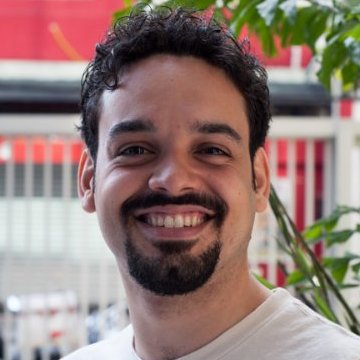
\includegraphics[width=4cm]{profile.jpg}
%  };
%\end{tikzpicture}

% In the aside, each new line forces a line break
\begin{aside}
  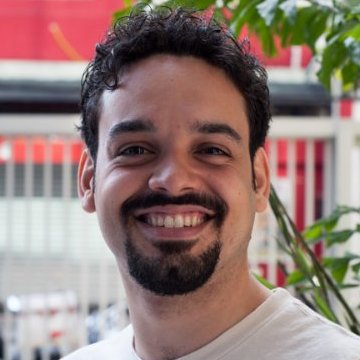
\includegraphics[width=4cm]{profile.jpg}
  \section{contact}
    R. Ministro Gastão Mesquita, 257
    05012-010 São Paulo
    Brasil
    ~
    +55 11 9 8393 2639
    %+33 \phantom{0}7 53 05 52 36
    {\footnotesize skype} guilherme\_nirev
    \href{mailto:guilherme@nirev.org}{guilherme@nirev.org}
    \href{http://nirev.org}{http://nirev.org}
  \section{languages}
    native portuguese
    fluent english
    basic french
  \section{programming}
    Elixir, Java, Ruby, Javascript, C, Python,
    HTML, css, bash
  \section{skills/tools}
    team leading, engineering manager,
    mysql, postgres,
    nginx, docker, DevOps,
    shell scripting
  \section{interests}
distributed systems, making a better world, data structures, music, martial arts, science fiction books
\end{aside}


\section{education}

\begin{entrylist}

\entry
  {2011–2014}
  {Master in Computer Science}
  {University of São Paulo - Brazil}{}
\entry
  {2005–2010}
  {B.Sc. in Computer Science}
  {Federal University of Espírito Santo - Brazil}{}
\end{entrylist}

\section{experience}

\workentry
    {September 2015}{*}
    {Senior Software Engineer at XERPA}
    {São Paulo - Brazil}
    {First Engineering hire. XERPA is a SAAS platform for HR, payroll, and benefits. We're building from zero with a 100\% functional stack: Elixir on the backend and ClojureScript+React on the front. We're also automating our infrastructure on AWS with Terraform and Ansible.}

\workentry
  {November 2012}{September 2015}
  {Team Lead (Search and Analytics) at Elo7}
  {São Paulo - Brazil}
  {A marketplace with high traffic and transaction volume. The stack was based on Java, Ruby and Scala on AWS infrastructure. A fast paced environment, with agile practices, and focusing on delivering fast with quality. We measured and logged using StatsD, Graphite, and NewRelic, and deployed constantly. I was leading the Search and Analytics Team: a small team using Solr, Kafka and Spark to improve search and real time reports, and responsible for its infrastructure and pipeline tools.}

\workentry
  {April 2012}{October 2012}
  {Intern at INRIA Paris-Roquencourt}
  {Rocquencourt, Île-de-France - France}
  {Research on fault-tolerance requirements for Wireless Sensor Networks macroprogramming.}

\workentry
  {March 2011}{September 2012}
  {Researcher for CHOReOS project}
  {University of São Paulo, São Paulo - Brazil}
  {Research and implementation involving: choreography analysis using graph metrics,
  dynamic adaptation techniques, implementation of a testing framework, and cloud computing.}

\workentry
  {August 2010}{February 2011}
  {Software Developer/Analyst at RR Sistema}
  {Vitória/ES - Brazil}
  {Porting their implementation of Brazilian DTV middleware to different platforms.
  Mainly programming in C/C++, with low-level and multimedia libraries (GStreamer, DirectFB, pthreads, osal, etc),
  and required knowledge of the Brazilian digital television standards.}

\workentry
  {January 2009}{December 2010}
  {Undergrad Intern at Multimedia and Network Research Lab}
  {Federal Univ. of Espiríto Santo, Vitória/ES - Brazil}
  {Working with the Brazilian DTV middleware; ported it for Android. }

\workentry
  {August 2008}{December 2008}
  {Undergrad Intern at Laboratory of Advanced Software SYstems (LASSY)}
  {University of Luxembourg - LU}
  {RESIST project: developed a prototype for SOA eHealth application with multiple services.}

% \workentry
%   {January 2008}{March 2008}
%   {Intern at CISA Trading S.A.}
%   {Trading company, São Paulo/SP - Brazil}
%   {Maintaining their internal software solution which manages all of the companies processes.
%   The system was written in the Progress4GL language.}

\workentry
  {March 2007}{December 2007}
  {Undergraduate Intern at NINFA laboratory}
  {Federal University of Espiríto Santo, Vitória/ES - Brazil}
  {Joint project with ESCELSA, state's electric power utility, building automated classifiers
  for finding frauds done by its clients. Used optimization heuristics, neural networks and clustering.
  Tools developed in Java, C++ and Matlab.}

\workentry
  {September 2006}{March 2007}
  {PHP Developer at Lettera Soluções}
  {Web developing company, Vitória/ES - Brazil}
  {}%Developing and managing web sites using CSS, (x)HTML, PHP, ASP, MySQL, PostgreSQL, as well as common Linux admin tools.}

\printbibsection{article}{article in peer-reviewed journal}
\printbibsectionpar{inproceedings}{international peer-reviewed conferences/proceedings}{notkeyword={brazil}}
\printbibsectionpar{inproceedings}{local peer-reviewed conferences/proceedings}{keyword={brazil}}
\printbibsection{misc}{other publications}
\printbibsection{report}{research reports}

\end{document}
